\chapter{Giới thiệu}
\label{Chapter1}

%Tóm tắt luận văn được trình bày nhiều nhất trong 24 trang in trên hai mặt giấy, cỡ chữ Times New Roman 11 của hệ soạn thảo Winword hoặc phần mềm soạn thảo Latex đối với các chuyên ngành thuộc ngành Toán.

%Mật độ chữ bình thường, không được nén hoặc kéo dãn khoảng cách giữa các chữ.
%Chế độ dãn dòng là Exactly 17pt.
%Lề trên, lề dưới, lề trái, lề phải đều là 1.5 cm.
%Các bảng biểu trình bày theo chiều ngang khổ giấy thì đầu bảng là lề trái của trang.
%Tóm tắt luận án phải phản ảnh trung thực kết cấu, bố cục và nội dung của luận án, phải ghi đầy đủ toàn văn kết luận của luận án.
%Mẫu trình bày trang bìa của tóm tắt luận văn (phụ lục 1).

\noindent Trong chương này, nhóm nghiên cứu sẽ phát biểu về bài toán xây dựng hệ thống gợi ý, cũng như đóng góp của nó cho cuộc sống của con người đến nay. Tiếp theo, ta sẽ trình bày về vấn đề dữ liệu thưa, một trong những vấn đề nhức nhối, bắt gặp nhiều nhất khi xây dựng một hệ thống gợi ý. Để giải quyết vấn đề này, phương pháp ``Học tự giám sát'' được sử dụng nhằm hạn chế tác động do dữ liệu thưa mang lại cho hệ thống. Phạm vi và phương pháp nghiên cứu sẽ được mô tả một cách tổng quát. Bố cục cũng sẽ được đề cập tới nhằm cho người đọc có thể nắm được toàn cảnh hoạt động nghiên cứu.

\section{Đặt vấn đề và Động lực}

\noindent Việc con người nhận được ngay những gợi ý, những quảng cáo từ các nền tảng ví dụ như mảng xã hội, sàn thương mại điện tử,... sau khi phát sinh lịch sử tương tác đã không còn quá xa lạ. Con người tương tác với sản phẩm dưới bất kỳ hình thức nào như xem sản phẩm, đặt mua sản phẩm, đánh giá sản phẩm,... đều rất đáng giá và được một số loại hệ thống ghi lại. Hệ thống gợi ý dựa trên lịch sử tương tác của người dùng hỗ trợ ra quyết định, cung cấp các gợi ý cho người dùng về những ``sản phẩm'' mà họ có thể cần. Ví dụ, sau khi xem một bộ phim trên Netflix, ta được gợi ý những bộ phim có thể loại tương tự, hay khi ta mua điện thoại, hệ thống sẽ gợi ý cho ta những phụ kiện điện thoại thường được mua kèm. Với những ``sản phẩm'' đúng, ta có thể mang lại trải nghiệm tốt cho người dùng, xa hơn là có thể thúc đẩy phát triển kinh doanh. Dưới kỷ nguyên 4.0, không gian tương tác ngày một lớn, trong khí đó người dùng có khuynh hướng chỉ tương tác với một phần rất nhỏ trong cơ sở dữ liệu. Điều này đã trở thành một động lực to lớn, thúc đẩy việc tìm ra một phương pháp hạn chế tác động tiêu cực đến từ chính bản thân dữ liệu này.

Bất kỳ dạng bài nào, ta cũng phải xác định rõ đầu vào, đầu ra (mục tiêu) của bài toán đó, mục tiêu của bài toán là gì. Vậy đầu vào, đầu ra của bài toán này là gì? Ở đầu vào, ta cần đưa cho hệ thống gợi ý lịch sử tương tác với ``sản phẩm'' của một hoặc nhiều người dùng. Đầu ra của hệ thống sẽ dự đoán về hành vi, ``sản phẩm'' của người dùng có thể thích hay cần ở hiện tại hoặc tương lai.

Bất kỳ bài toán nào, cũng tồn tại những vấn đề của riêng nó. Bài toán hệ thống gợi ý đang phải giải quyết một số vấn đề  như dữ liệu thưa. Trong ngữ cảnh của hệ thống gợi ý, đa phần người dùng sẽ chỉ tương tác với một phần rất nhỏ trong một lượng lớn các ``sản phẩm'' tồn tại trong cơ sở dữ liệu. Điều này sẽ gây khó khăn cho việc tìm ra những người dùng ``giống nhau''. Bên cạnh đó, hành vi của người dùng chịu ảnh hưởng bởi tác động của rất nhiều yếu tố. Tập hợp những điều đó lại, có thể dẫn đến việc sai lệch trong quá trình đưa ra gợi ý.

Bài toán xây dựng hệ thống gợi ý là bài toán không mới, tuy nhiên nó cũng chỉ mới nở rộ cách đây không lâu \cite{survey:sota-rec-system}, và cũng còn rất nhiều tiềm năng để phát triển. Học sâu đã mở ra một chương mới cho bài toán xây dựng hệ thống gợi ý, điều này minh chứng bằng việc sự phát triển nhanh chóng mà các mô hình học sâu mang lại dạo thời gian gần đây. Mạng học sâu đồ thị, học tăng cường, học tự giám sát là một vài chủ đề trong những chủ đề đang nhận được khá nhiều quan tâm hiện tại. Học tự giám sát chủ đề nghiên cứu chính được trình bày trong khóa luận này.

Học giám sát (Supervised Learning) cần một lượng lớn dữ liệu được gán nhãn cẩn thận để đem lại hiệu quả tốt. Việc này đòi hỏi một lượng lớn thời gian, tiền bạc để gán nhãn và điều này quả thực là rất tốn kém. Trong khi đó, lượng dữ liệu chưa được gán nhãn thì lại rất nhiều và liên tục được sinh ra, nếu ta chăm chăm vào việc làm sao để gán nhãn thì sẽ không kịp các tiến trình học. Gần đây, Học tự giám sát (Self-supervised Learning) là một hướng nghiên cứu mới được đưa ra và nhận được khá nhiều sự quan tâm, có tiềm năng giải quyết/hạn chế một phần các vấn đề của hệ thống gợi ý (ví dụ điển hình như dữ liệu thưa).

Bằng cách sử dụng học tự giám sát, ta có thể tận dụng lượng dữ liệu không gán nhãn, học từ chính những đặc trưng bên trong của dữ liệu, cải tiến hiệu quả của toàn bộ hệ thống. Học tự giám sát được áp dụng trong rất nhiều lĩnh vực nghiên cứu, và là hướng nghiên cứu đang còn rất mới kể cả trong lĩnh vực xử lý ảnh hay ngôn ngữ tự nhiên, việc áp dụng mô hình học này vào bài toán hệ thống gợi ý lại càng mới hơn. Ở phần tiếp theo, mục tiêu nghiên cứu của khóa luận sẽ được trình bày kỹ hơn.

\section{Mục tiêu nghiên cứu}

\noindent Như đã đề cập, học tự giám sát là một trong những phương pháp đáng hứa hẹn với hi vọng giải quyết được các vấn đề còn vướng phải của hệ thống gợi ý ở hiện tại và tương lai. 

Với đề tài này, ta cần biết được tình hình nghiên cứu về mạng học sâu đồ thị cho hệ thống gợi ý cũng như việc áp dụng học tự giám sát vào bài toán này trong thời gian gần đây. Qua đó biết được các hướng nghiên cứu đã và đang được hướng tới, hướng nào tốt hoặc chưa tốt ở điểm nào, các vấn đề đã giải quyết được cũng như các vấn đề vẫn cần phải quyết trong tương lai.

Điều căn bản nhất, ta cần hiểu rõ được lý thuyết xoay quanh bài toán học giám sát trên mạng học sâu đồ thị cho hệ thống gợi ý. Đầu tiên là về hệ thống gợi ý; tiếp theo là về mạng học sâu đồ thị - một loại mạng học sâu đã và đang được nhiều công trình nghiên cứu hướng tới áp dụng, cách áp dụng mạng học sâu này lên hệ thống gợi ý như thế nào; ta cũng biết được có những cách nào để áp dụng mô hình học tự giám sát - một phương pháp được áp dụng trên mạng học sâu không chỉ trên hình ảnh, văn bản mà thậm chí có thể sử dụng với đồ thị một cách hiệu quả. Từ đó có thể nắm vững kiến thức nền tảng một cách có hệ thống.

Không kém phần quan trọng, ta cần nghiên cứu và cài đặt những gì nghiên cứu được. Cụ thể, đề tài này sẽ đi theo ý tưởng chính của Wu \cite{SGL} và tiến hành cài đặt lại học tự giám sát trên mạng học sâu đồ thị, nhằm chứng minh được hiệu quả mang lại của phương pháp này vào bài toán hệ thống gợi ý. Bên cạnh đó, ta cũng sẽ tiến hành tìm hiểu, thử nghiệm một số cải tiến nhằm giải quyết những điểm chưa tốt của mô hình hiện tại. Việc này nhằm nhìn nhận lại vấn đề và giải quyết một phần nào đó những hạn chế mà hướng nghiên cứu hiện tại đang gặp phải. Từ đó mở ra cơ hội khai thác sâu hơn hoặc tìm ra được các hướng nghiên cứu mới hơn, hiệu quả hơn trong bài toán hệ thống gợi ý.

\section{Phạm vi nghiên cứu}

\noindent 3 bộ dữ liệu thường được sử dụng trong các đề tài nghiên cứu về mạng học sâu đồ thị cho hệ thống gợi ý được đề tài chọn để tiến hành thí nghiệm:
\begin{itemize}
    \item[(1)] Yelp 2018: bộ dữ liệu của Yelp, chứa thông tin về doanh nghiệp, người dùng, và đánh giá của người dùng về các doanh nghiệp đó.

    \item[(2)] Amazon Book: thông tin đánh giá của người dùng từ Amazon trong khoảng từ năm 1996 đến 2014.

    \item[(3)] Alibaba iFashion: bộ dữ liệu công khai của Alibaba, gồm các sản phẩm thời trang của trang bán hàng online và các tương tác của người dùng.
\end{itemize}
Chi tiết cụ thể về các bộ dữ liệu sẽ được đề cập ở phần sau.

Đề tài sẽ tập trung về việc giải thích học tự giám sát trên mạng học sâu đồ thị được áp dụng vào hệ thống gợi ý. Bên cạnh đó, một số thí nghiệm sẽ được tiến hành nhằm cải tiến thêm dựa trên những vấn đề đang gặp phải của hệ thống bên trên.

Trong suốt quá trình thực hiện đề tài, những hạn chế của nghiên cứu sẽ được thừa nhận, giải quyết. Những kết quả sẽ được giải thích và thảo luận những yếu tố tác động. Các nghiên cứu trong tương lai có thể  được tiến hành mở rộng dựa trên kết quả của nghiên cứu này và giải quyết những thiếu sót mà hiện tại vẫn chưa giải quyết được. Nhìn chung, nghiên cứu này sẽ cung cấp những kiến thức nền tảng, nâng cao hiểu biết về những tiềm năng còn khai phá được trong lĩnh vực hệ thống gợi ý nhằm nâng cao hiệu quả của mô hình này nói chung và hướng nghiên cứu, áp dụng mô hình học học tự giám sát vào hệ thống này nói riêng.

\section{Phương pháp nghiên cứu}

\noindent Như ta có đề cập rằng việc gán nhãn cho bộ dữ liệu quả thực là một điều cực kỳ tốn kém. Việc gán nhãn cho bài toán sử dụng bộ dữ liệu dạng hình ảnh, văn bản có thể sẽ dễ dàng hơn so với bài toán hệ thống gợi ý. Lúc này, dữ liệu được tạo ra bởi chính bản thân người dùng, người dùng tương tác với sản phẩm và để lại đánh giá của riêng mình. Tuy nhiên, đa số người dùng chỉ tương tác với một phần nhỏ các mục/vật phẩm so với toàn bộ vật phẩm mà họ có thể tương tác tới. Vì vậy, vấn đề về dữ liệu huấn luyện vẫn luôn là một chướng ngại gây cản trở các mô hình gợi ý học sâu có thể đạt được tiềm năng của nó.

Tất nhiên là không phải lúc nào dữ liệu cũng được gán nhãn sẵn. Trong nhiều trường hợp thực tế, ta phải đối mặt với một lượng lớn dữ liệu không nhẵn (có thể là chưa gán nhãn hoặc thậm chí không thể gán nhãn). Với học tự giám sát, mô hình có thể học được từ chính những đặc trưng bên trong của dữ liệu, từ đó cải thiện độ chính xác của mô hình. 

Để cải thiện hệ thống gợi ý, ta có thể áp dụng nó đồng thời với tác vụ học tự giám sát (self-supervised learning). Cụ thể, mô hình sẽ được huấn luyện bằng cách để tác vụ gợi ý đóng vai trò chính; học tự giám sát, cụ thể hơn là học tương phản (contrastive learning) với vai trò bổ trợ nhằm tối ưu cho mô hình gợi ý cổ điển. Để áp dụng được học tương phản, ta sẽ cần rất nhiều dữ liệu và hiển nhiên bộ dữ liệu gốc (bộ dữ liệu hạn chế) mà ta có ban đầu sẽ không đáp ứng được điều này. Tăng cường dữ liệu (data augmentation) -- một kỹ thuật nhằm tăng thêm dữ liệu từ chính dữ liệu mà ta hiện có, được áp dụng rất nhiều trên dữ liệu dạng hình ảnh, văn bản cũng mang lại kết quả khá khả quan trong các công trình nghiên cứu dạo gần đây trên dữ liệu dạng đồ thị. Không khác về mặt ý tưởng, khi áp dụng đồ thị, tăng cường dữ liệu hoạt động bằng cách tạo ra các biến thể (view) khác nhau từ đồ thị gốc ban đầu, các biến thể này vẫn giữ đuợc đặc trưng, cấu trúc từ đồ thị gốc. Với các biến thể mới được tạo ra này, ta có thể học được cách biểu diễn một cách tốt hơn từ việc khiến các biến thể khác nhau của cùng một node tiến lại gần nhau, khác node đẩy ra xa nhau. Từ đó, cải thiện hiệu suất chung cho toàn bộ hệ thống.

\begin{figure}[H]
    \centering
    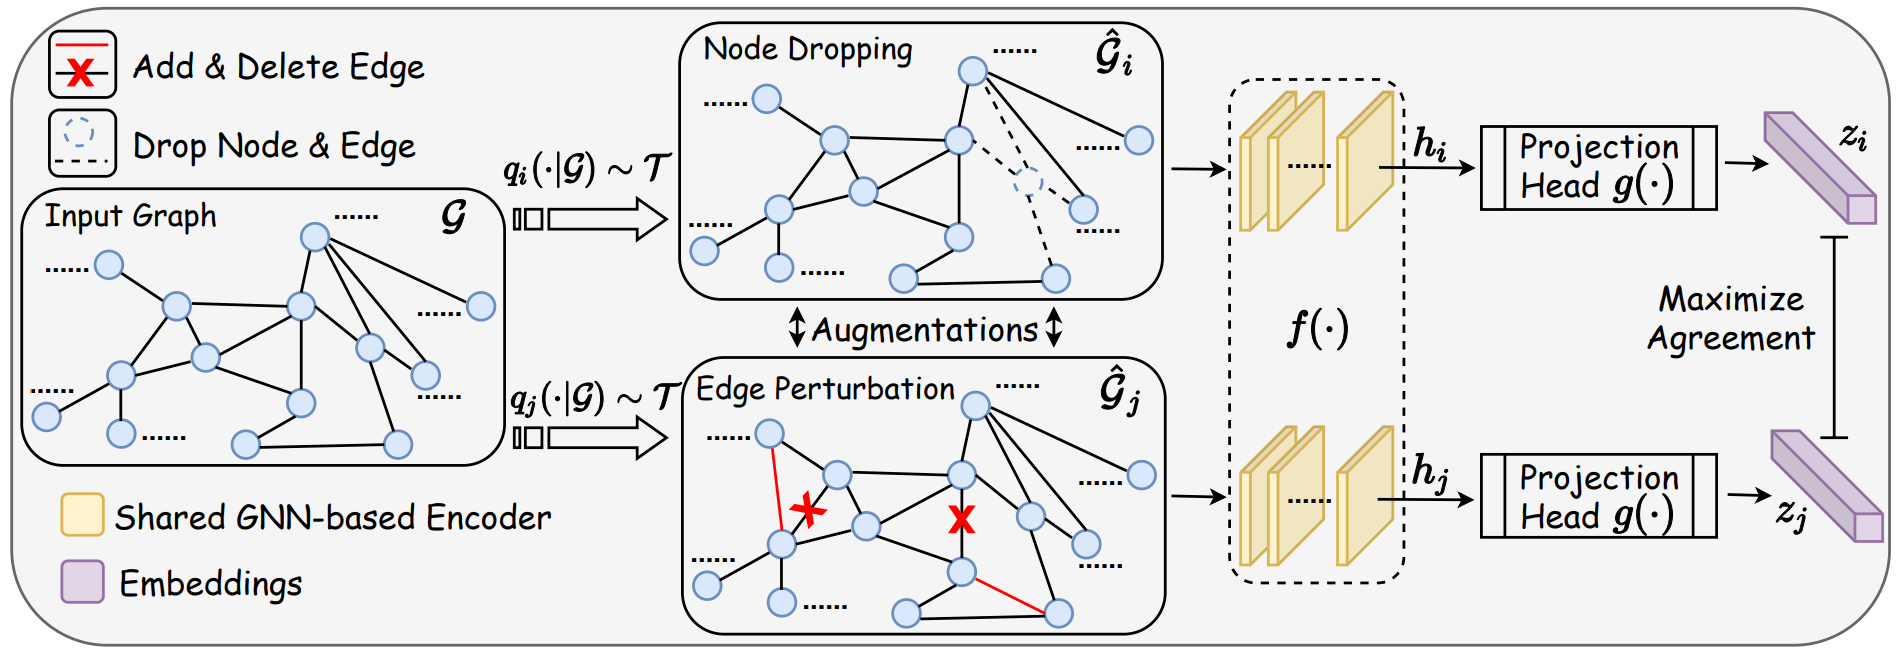
\includegraphics[scale=0.31]{images/Chapter1/graph-contrastive-learning.png}
    \caption{Ví dụ về việc tạo ra các view dẫn tới việc tác dộng đến học biểu diễn.}
\end{figure}

\section{Bố cục}

\noindent Ở chương này, ta cũng đã trình bày về vai trò của hệ thống gợi ý trong cuộc sống, cũng như cho thấy được rằng, hệ thống gợi ý nói chung và học tự giám sát trên hệ thống gợi ý nói riêng vẫn còn rất mới và thực sự có rất nhiều tiềm năng để đầu tư nghiên cứu. Phần còn lại của khóa luận sẽ trình bày theo thứ tự như sau:
\begin{itemize}
    \item[] \textbf{Chương 2}: Trình bày các kiến thức nền tảng về hệ thống gợi ý, mạng học sâu đồ thị, tăng cường dữ liệu và mô hình Học tự giám sát (Self-supervised Learning).
    
    \item[] \textbf{Chương 3}: Trình bày về việc áp dụng học tự giám sát lên mạng học sâu đồ thị cho hệ thống gợi ý. Đây là phần quan trọng nhất của khóa luận, cụ thể:
        \begin{itemize}
            \item Tăng cường dữ liệu trên dữ liệu dạng đồ thị: Trình bày các cách phổ biến để giải quyết tình trạng vấn đề ``đói dữ liệu'' trên mạng học sâu đồ thị.

            \item Những thành tựu của mạng học sâu đồ thị đã được chứng minh qua rất nhiều công trình nghiên cứu. Trình bày cách áp dụng mạng này vào cho hệ thống gợi ý.
            
            \item Phần cuối và cũng là phần tổng hợp lại để đúc kết toàn bộ ý tưởng của việc áp dụng mô hình học ``Học tự giám sát'' vào mạng học sâu đồ thị cho hệ thống gợi ý. 
        \end{itemize}
    
    \item[] \textbf{Chương 4}: Trình bày về thí nghiệm đã thực hiện và các kết quả thu được trong suốt quá trình nghiên cứu.
    
    \item[] \textbf{Chương 5}: Tổng kết lại những gì đã nghiên cứu được và những hướng phát triển tiềm nằng trong tương lai.
\end{itemize}
